\section{(3.2)}

% template of how to format
% \textit{An HVAC engineer has determined the amount of air per room required to maintain a comfortable and quiet space}
% \begin{table}[H]
% \centering
% \begin{tabular}{cc}
% \toprule
% Office Space & Heating Air Requirement (cfm) \\ 
% \midrule
% Office 204 & 330 \\
% Office 205 & 470 \\
% Office 206 & 190 \\
% Office 207 & 520 \\
% \bottomrule
% \end{tabular}
% \end{table}
% \paragraph{a)} \textit{The architect has requested the design of a round ductwork system (duct material, sizes of round duct, necessary fittings, including diffusers, in a ductwork system, and the 2D system layout). You can use the dimensions of rooms to estimate the duct lengths. Note: You are free to design a duct system layout (No specific guidance needs to follow).}\\
% \subsection{Assumptions:}
% \begin{enumerate}
%     \item $v_{\text{max}} = 1200$ fpm since the air is to be quiet for the office space.
%     \item Round ductwork system
%     \item $\Delta P$ unknown $\to$ friction loss = 0.1'' wg/100 ft.
%     \item Diffusers are to be placed in each room. Assume that the pressure loss across the diffuser is 0.05'' wg. (Table 2.2).
%     \item Galvanized steel duct material is used (common in air ducts).
%     \item Bellmouth entrance from supply fan and diffuser entrance are to be considered.
%     \item The elbow is pleated 90$^\circ$.
% \end{enumerate}

% new question
% Cooling water is pumped from a reservoir to equipment at a construction site through a 4-
% inch inner diameter aluminum pipe system, as shown below. The discharge pipe, 566 feet in
% length, is connected to a globe valve. Note that aluminum pipes have an average roughness
% similar to drawn tubing. The discharge pipe also includes 15 joints (each with a loss
% coefficient Kjoint=1, though not shown in the figure). The required flow rate is 600 gpm, and
% the water must exit the spray nozzle (a component with a reduced cross-sectional area, K=14)
% at 120 fps. The suction pipe is a short 5-foot section (indicated in the figure), with the pump
% positioned 0.5 feet above the water surface. Please address the following:
% (1) Estimate the required motor power considering a pump efficiency of 80%.
% (2) Assess whether cavitation will occur if the NPSHR for this pump is 20 ft.
% Note: the indicated lengths are not to scale.0.5 FT

\textit{Cooling water is pumped from a reservoir to equipment at a construction site through a 4-inch inner diameter aluminum pipe system, as shown below. The discharge pipe, 566 feet in length, is connected to a globe valve. Note that aluminum pipes have an average roughness similar to drawn tubing. The discharge pipe also includes 15 joints (each with a loss coefficient Kjoint=1, though not shown in the figure). The required flow rate is 600 gpm, and the water must exit the spray nozzle (a component with a reduced cross-sectional area, K=14) at 120 fps. The suction pipe is a short 5-foot section (indicated in the figure), with the pump positioned 0.5 feet above the water surface. Please address the following:}

\paragraph{(1)} \textit{Estimate the required motor power considering a pump efficiency of 80\%.}
\paragraph{(2)} \textit{Assess whether cavitation will occur if the NPSHR for this pump is 20 ft.}

\begin{figure}[H]
    \centering
    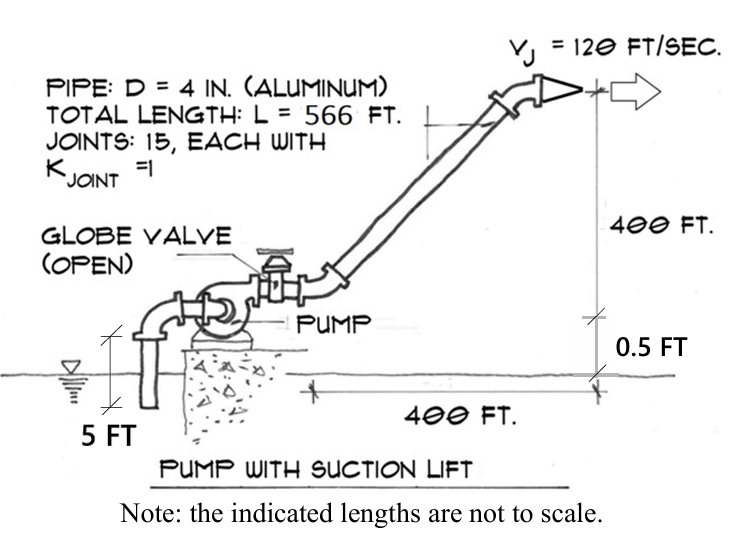
\includegraphics[width=0.9\textwidth]{Questions/Figures/Q1 Diagram.png}
\end{figure}

\subsection{Assumptions}
\begin{enumerate}
    \item All pipe fittings are flanged
    \item Water is room temperature, 70$^\circ$F
    \item Two 45$^\circ$ bends and two 90$^\circ$ bends are used
    \item The reservoir is sufficiently large that the water velocity is negligible
\end{enumerate}

\subsection{Sketches}
\begin{figure}[H]
    \centering
    
\includegraphics[width=0.9\textwidth]{Questions/Figures/Q1 Sketch.png}
\end{figure}

\subsection{Analysis}
\subsubsection{Pipe Friction}
First the properties of water can be found from Table A-9E at 70$^\circ$F:
\begin{align*}
    \mu = 6.556 \times 10^{-4} \; \text{lbm/ft-s} \quad \text{and} \quad \rho = 62.30 \; \text{lbm/ft}^3 \\
    P_{\text{vapour}} = 0.3632 \; \text{psia}
\end{align*}
The Reynolds number can be calculated as:
\begin{align*}
    \text{Re} = \frac{\rho v D}{\mu} = \frac{4 \rho \dot{V}}{\pi \mu D} = \frac{4 \cdot 62.30 \cdot 600 \text{gpm}}{\pi \cdot 6.556 \times 10^{-4} \cdot \frac{4}{12} \; \text{ft}} \cdot \frac{1 \; \text{ft}^3}{7.48 \; \text{gallons}} \cdot \frac{1 \; \text{min}}{60 \; \text{s}} = 4.85 \times 10^5
\end{align*}
This flow is turbulent.

The relative roughness is
\begin{align*}
    \frac{\varepsilon}{D} = \frac{0.000005 \; \text{ft}}{\frac{4}{12} \; \text{ft}} = 0.000015 = 1.5 \times 10^{-5}
\end{align*}
From the Moody diagram, the friction factor is $f = 0.014$.
\begin{figure}[H]
    \centering
    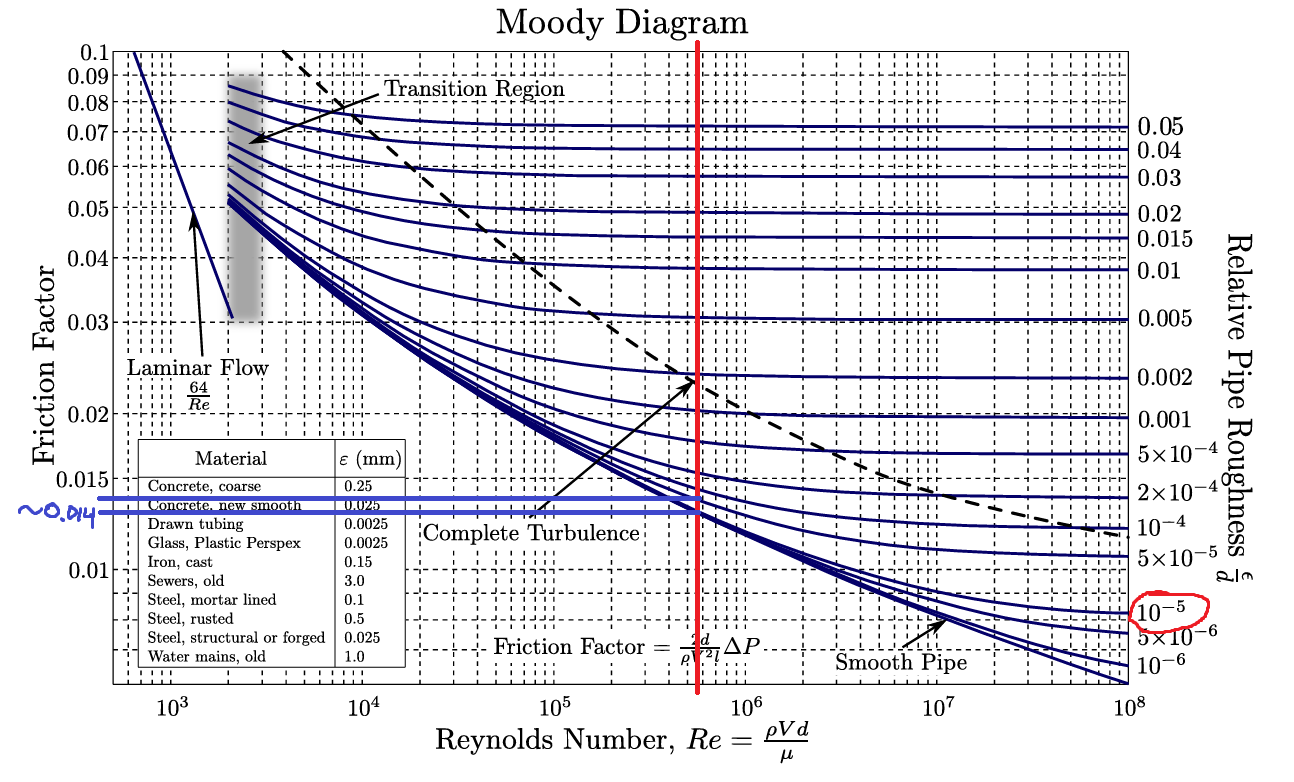
\includegraphics[width=0.9\textwidth]{Questions/Figures/Q1 Moody.png}
\end{figure}

\subsection{Outlet Reynolds}
We know the outlet velocity is 120 fps, and that
\begin{align*}
    \dot{V}    & = \pi \frac{D^2}{4} v                                                                                                                                                                                                     \\
    \implies D & = \sqrt{\frac{4 \dot{V}}{\pi v}} = \sqrt{\frac{4 \cdot 600 \text{gpm}}{\pi \cdot 120 \text{fps}}} \cdot \frac{1 \; \text{ft}^3}{7.48 \; \text{gallons}} \cdot \frac{1 \; \text{min}}{60 \; \text{s}} = 0.119 \; \text{ft}
\end{align*}
Therefore the Reynolds number at the outlet is
\begin{align*}
    \text{Re} = \frac{4 \rho v}{\pi \mu D} = \frac{4 \cdot 62.30 \cdot 120}{\pi \cdot 6.556 \times 10^{-4} \cdot 0.119} = 1.36 \times 10^6
\end{align*}
This flow is also turbulent, $\alpha_2 = 1.06$.

\subsection{Energy Equation}
The energy equation can be written as
\begin{align*}
    h_\text{pump} & = \left(\frac{P_2}{\rho g} + \alpha_2 \frac{v_2^2}{2g} + z_2\right) - \left(\frac{P_1}{\rho g} + \cancelto{0}{\alpha_1 \frac{v_1^2}{2g}} + \cancelto{0}{z_1}\right) + H_{\text{lT}} \\
                  & = \cancelto{0}{\frac{P_2 - P_1}{\rho g}} + \alpha_2 \frac{v_2^2}{2g} + z_2 + H_{\text{lT}}                                                                                          \\
                  & = \alpha_2 \frac{v_2^2}{2g} + z_2 + H_{\text{lT}}
\end{align*}
Where
\begin{align*}
    H_{\text{lT}} & = \\frac{v_\text{pump}^2}{2g} \left(f \frac{L}{D} + \sum K_L\right)
\end{align*}

From Table A.14 for losses,
\begin{align*}
    K_{\text{globe}}    & = 6 \quad K_{\text{exit}} = 1       \\
    K_{\text{45}^\circ} & = 0.19 \quad K_{\text{nozzle}} = 14 \\
    K_{\text{inlet}}    & = 0.78 \quad K_{\text{joint}} = 1   \\
    K_{\text{90}^\circ} & = 0.3
\end{align*}
Then,
\begin{align*}
    \sum K_L & = K_{\text{globe}} + K_{\text{exit}} + 2K_{\text{45}^\circ} + K_{\text{nozzle}} + K_{\text{inlet}} + 15K_{\text{joint}} + 2K_{\text{90}^\circ} \\
             & = 6 + 1 + 2(0.19) + 14 + 0.78 + 15 + 2(0.3) = 37.76
\end{align*}
Then,
\begin{align*}
    H_{\text{lt}} & = \frac{8 Q^2}{\pi^2 g D^4} \left(f \frac{L}{D} + \sum K_L\right)                                                                                                                                                          \\
                  & = \frac{8 \cdot 600^2}{\pi^2 \cdot 32.2 \cdot 0.119^4} \cdot \left(\frac{1 \; \text{ft}}{7.48 \; \text{gal}} \cdot \frac{1 \; \text{min}}{60 \; \text{s}}\right)^2 \cdot \left(0.014 \cdot \frac{566}{4/12} + 37.76\right) \\
                  & = 226  \; \text{ft}
\end{align*}
and
\begin{align*}
    h_{\text{pump}} & = \alpha_2 \frac{v_2^2}{2g} + z_2 + H_{\text{lT}}                      \\
                    & = 1.06 \cdot \frac{120^2}{2 \cdot 32.2} + 400 + 226 = 863 \; \text{ft}
\end{align*}

\subsubsection{Power}
The power required for $\eta = 0.80$ is
\begin{framed}
    \begin{align*}
        \text{bhp} & = \frac{\rho \dot{V} h_{\text{pump}}}{\eta}                                                                                                                    \\
                   & = \frac{62.30 \cdot 600 \cdot 863}{0.80} \cdot \frac{1 \; \text{ft}^3}{7.48 \; \text{gallons}} \cdot \frac{1 \; \text{min}}{60 \; \text{s}} = 163 \; \text{hp}
    \end{align*}
\end{framed}

\subsubsection{Cavitation}
NPSH is defined as
\begin{align*}
    \text{NPSH} = \left(\frac{P}{\rho g} + \frac{v_\text{avg, in}^2}{2g}\right)_{\text{pump, in}} - \frac{P_\text{vapour}}{\rho g}
\end{align*}
We need to determine the pressure at the pump inlet. By energy balance,
\begin{align*}
    \left(\frac{P_i}{\rho g} + \alpha_i \frac{v_i^2}{2g} + z_i\right) + H_{\text{lT}} = \left(\frac{P_1}{\rho g} + \alpha_1 \frac{v_1^2}{2g} + z_1\right)
\end{align*}
Assuming $v_1 = v_i$ and defining $z_1 = 0$,
\begin{align*}
    \frac{P_i}{\rho g} = \frac{P_\text{atm}}{\rho g} - z_i - H_{\text{lT}}
\end{align*}
$H_{\text{lT}}$ is
\begin{align*}
    H_{\text{lT}} & = \frac{v_i^2}{2g} \left(f \frac{L}{D} + \sum K_L\right) \\
\end{align*}
where,
\begin{align*}
    \sum K_L & = K_\text{inlet} + 2K_{90^\circ} \\
             & = 0.78 + 2(0.3) = 1.38           \\
\end{align*}
and
\begin{align*}
    v_1 = v_i & = \frac{\dot{V}}{\pi D^2}                                                                                                                   \\
              & = \frac{4 \cdot 600}{\pi \cdot (4/12)^2} \cdot \frac{1 \; \text{ft}^3}{7.48 \; \text{gallons}} \cdot \frac{1 \; \text{min}}{60 \; \text{s}} \\
              & = 15.31 \; \text{fps}
\end{align*}
Then,
\begin{align*}
    H_{\text{lT}} & = \frac{15.31^2}{2 \cdot 32.2} \left(0.014 \cdot \frac{5}{4/12} + 1.38\right) = 5.79 \; \text{ft}
\end{align*}
\begin{framed}
    Then NPSH,
    \begin{align*}
        \text{NPSH} & = \frac{P_\text{atm} - P_\text{vapour}}{\rho g} - z_i - H_{\text{lT}}                                                                                             \\
                    & = \frac{14.7 - 0.3632}{62.30 \cdot 32.2} \cdot \frac{32.2 \text{lb ft}^2\text{/s}}{1 \text{lbf}} \cdot \left(\frac{12\text{in}}{1\text{ft}}\right)^2 - 0.5 - 5.79 \\
                    & = 26.8 \; \text{ft}
    \end{align*}
    Since NPSH is greater than NPSHR, cavitation will not occur.
\end{framed}

\subsection{Conclusion}
Cavitation will not occure in the pump and the required motor power is 163 hp assuming an efficiency of 80\%. A strainer or foot valve would be a good addition tothe inlet suction pipe. The fluid velocity is also quite high, so a larger pipe diameter may be considered to reduce the velocity and pressure drop.

\